\chapter{Results}
\label{chap:results}
\lhead{\emph{Results}}

\section{Introduction}

This chapter presents the results from our earlier systematic approach. By analysing the OCR performance on pre-processed image datasets, we aim to confirm that image pre-processing improves OCR effectiveness on sensor reading images. Each section discusses the results, highlighting the impact of the methodologies and paving the way for further discussion.

\newpage
\section{First Sprint - Global Generic}

\begin{table}[h]
    \centering
    \caption{OCR Performance First Sprint}
    \label{tab:first_sprint_results}
    \begin{tabular}{|l|c|c|c|}
        \hline
        \textbf{Folder} & \textbf{Total Count} & \multicolumn{2}{c|}{\textbf{Tesseract}}                     \\
        \hline
                        &                      & \textbf{Read}                           & \textbf{Not Read} \\
        \hline
        A               & 165                  & 0                                       & 165               \\
        B               & 26                   & 5                                       & 21                \\
        C               & 10                   & 0                                       & 10                \\
        D               & 27                   & 0                                       & 27                \\
        E               & 10                   & 0                                       & 10                \\
        F               & 15                   & 0                                       & 15                \\
        G               & 19                   & 3                                       & 16                \\
        H               & 14                   & 3                                       & 11                \\
        \hline
    \end{tabular}
\end{table}

\vspace{1in}

% Of the 286 images 11 were read making a 3.85\% read count.


\begin{figure}[ht]
    \centering
    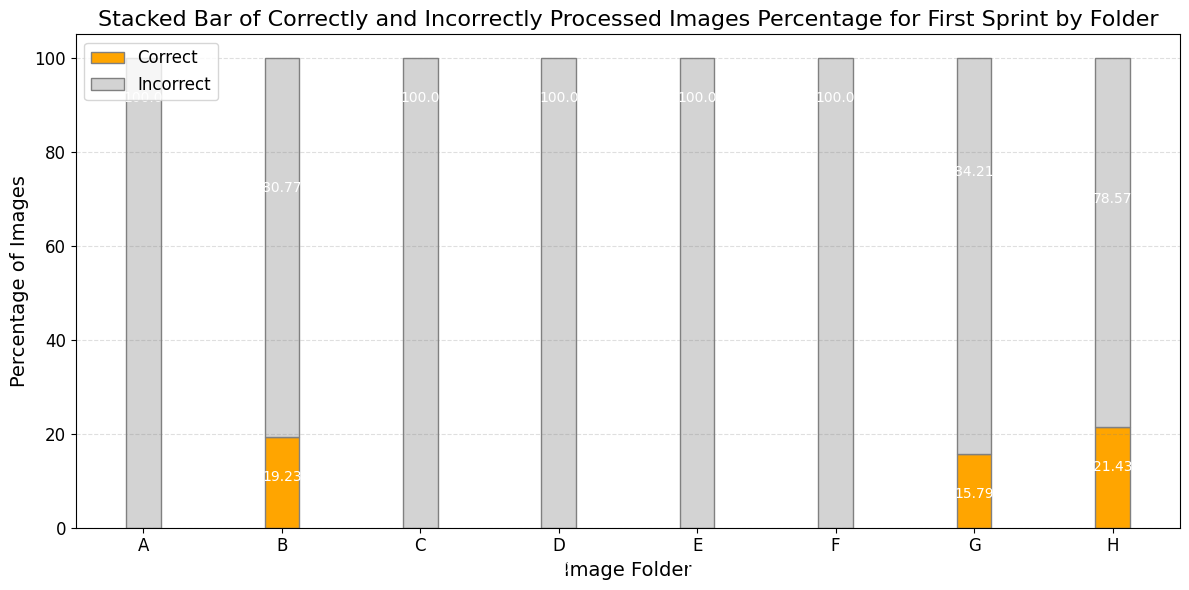
\includegraphics[width=0.7\textwidth]{Figures/Results/tesseract_sprints_one.png}
    \caption[Tesseract First Sprint Across Folders]{Tesseract First Sprint Across Folders}
    \label{fig:Tesseract First Sprint Across Folders}
\end{figure}

\vspace{1in}

\textbf{Observations}:
The chart demonstrates that most images across all folders were processed inaccurately. While Folders B, G, and H had some images processed correctly—with Folder H leading in accuracy—Folders A, C, D, E, and F recorded a complete lack of successful processing. This emphasizes the need for refining the image pre-processing algorithms.

\newpage

\section{Second Sprint - Global Generic Analysis Resized}


\begin{table}[h]
    \centering
    \caption{OCR Performance for Second Sprint}
    \label{tab:second_print_results}
    \begin{tabular}{|l|c|c|c|}
        \hline
        \textbf{Folder} & \textbf{Total Count} & \multicolumn{2}{c|}{\textbf{Tesseract}}                     \\
        \hline
                        &                      & \textbf{Read}                           & \textbf{Not Read} \\
        \hline
        A               & 165                  & 1                                       & 164               \\
        B               & 26                   & 12                                      & 14                \\
        C               & 10                   & 0                                       & 10                \\
        D               & 27                   & 0                                       & 27                \\
        E               & 10                   & 2                                       & 8                 \\
        F               & 15                   & 2                                       & 13                \\
        G               & 19                   & 5                                       & 14                \\
        H               & 14                   & 7                                       & 7                 \\
        \hline
    \end{tabular}
\end{table}

\vspace{1in}

\begin{figure}[ht]
    \centering
    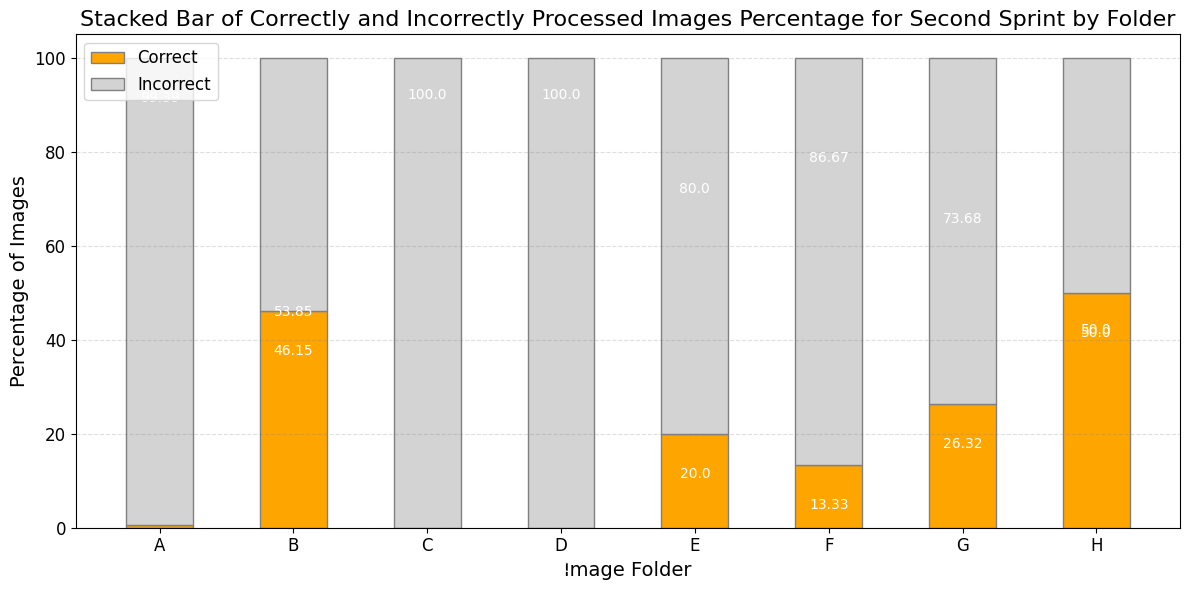
\includegraphics[width=0.7\textwidth]{Figures/Results/tesseract_sprints_two.png}
    \caption[Tesseract Second Sprint Across Folders]{Tesseract Second Sprint Across Folders}
    \label{fig:Tesseract Second Sprint Across Folders}
\end{figure}

\vspace{1in}

\textbf{Observations}:The second sprint shows improvement in image processing across more folders, with larger orange sections. Folders B, E, F, G and H have a higher percentage of correctly processed images. Folders A, C, and D still have 100\% or near, incorrectly processed images, indicating that the image pre-processing algorithms needs to be improved further to achieve better results.

\newpage

\section{Third Sprint - Analysis Tesseract Separate Folders}

\begin{table}[h]
    \centering
    \caption{OCR Performance for Different Folders}
    \label{tab:third_sprint_results}
    \begin{tabular}{|l|c|c|c|}
        \hline
        \textbf{Folder} & \textbf{Total Count} & \multicolumn{2}{c|}{\textbf{Tesseract}}                     \\
        \hline
                        &                      & \textbf{Read}                           & \textbf{Not Read} \\
        \hline
        A               & 165                  & 70                                      & 90                \\
        B               & 26                   & 12                                      & 14                \\
        C               & 10                   & 3                                       & 7                 \\
        D               & 27                   & 16                                      & 11                \\
        E               & 10                   & 10                                      & 0                 \\
        F               & 15                   & 1                                       & 14                \\
        G               & 19                   & 12                                      & 7                 \\
        H               & 14                   & 13                                      & 1                 \\
        \hline
    \end{tabular}
\end{table}
\vspace{1in}
\begin{figure}[ht]
    \centering
    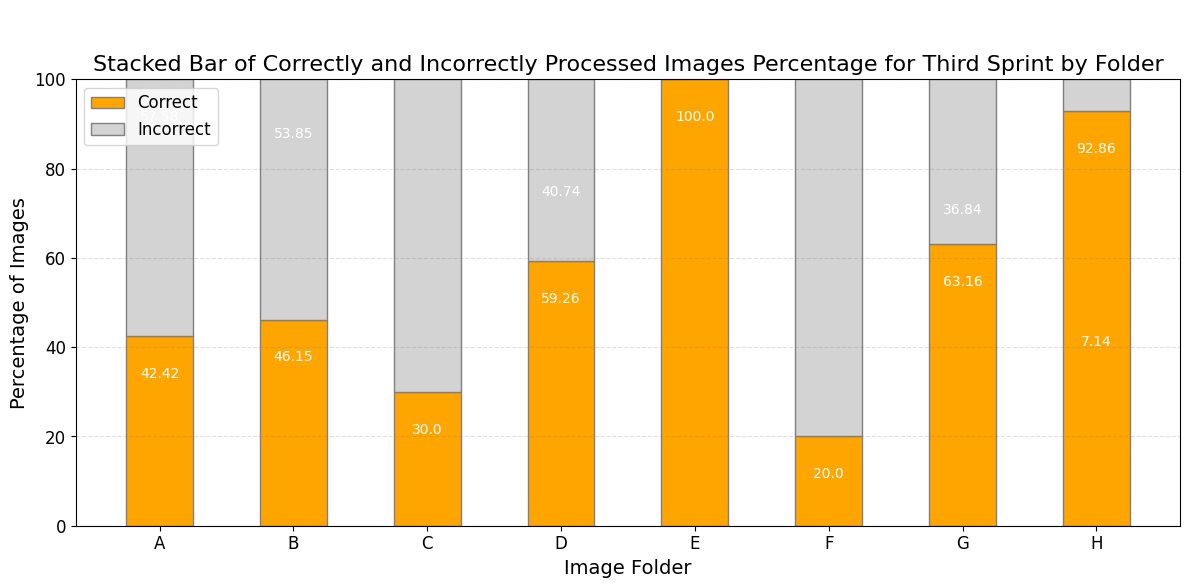
\includegraphics[width=0.7\textwidth]{Figures/Results/tesseract_sprints_three.png}
    \caption[Tesseract Third Sprint Across Folders]{Tesseract Third Sprint Across Folders}
    \label{fig:Tesseract Third Sprint Across Folders}
\end{figure}

\vspace{1in}

\textbf{Observations}: Most folders now show a high percentage of correctly processed images. Folders E, and F are particularly successful, with close to or even 100\% correctness. Folders G and I still have a proportion of incorrectly processed images, but their performance has improved significantly from the earlier sprints. Folder H has also seen improvement, but its rate of correctly processed images is slightly lower than the others.

\newpage

\section{Visualisation of Tesseract Sprint Performance}

\begin{figure}[ht]
    \centering
    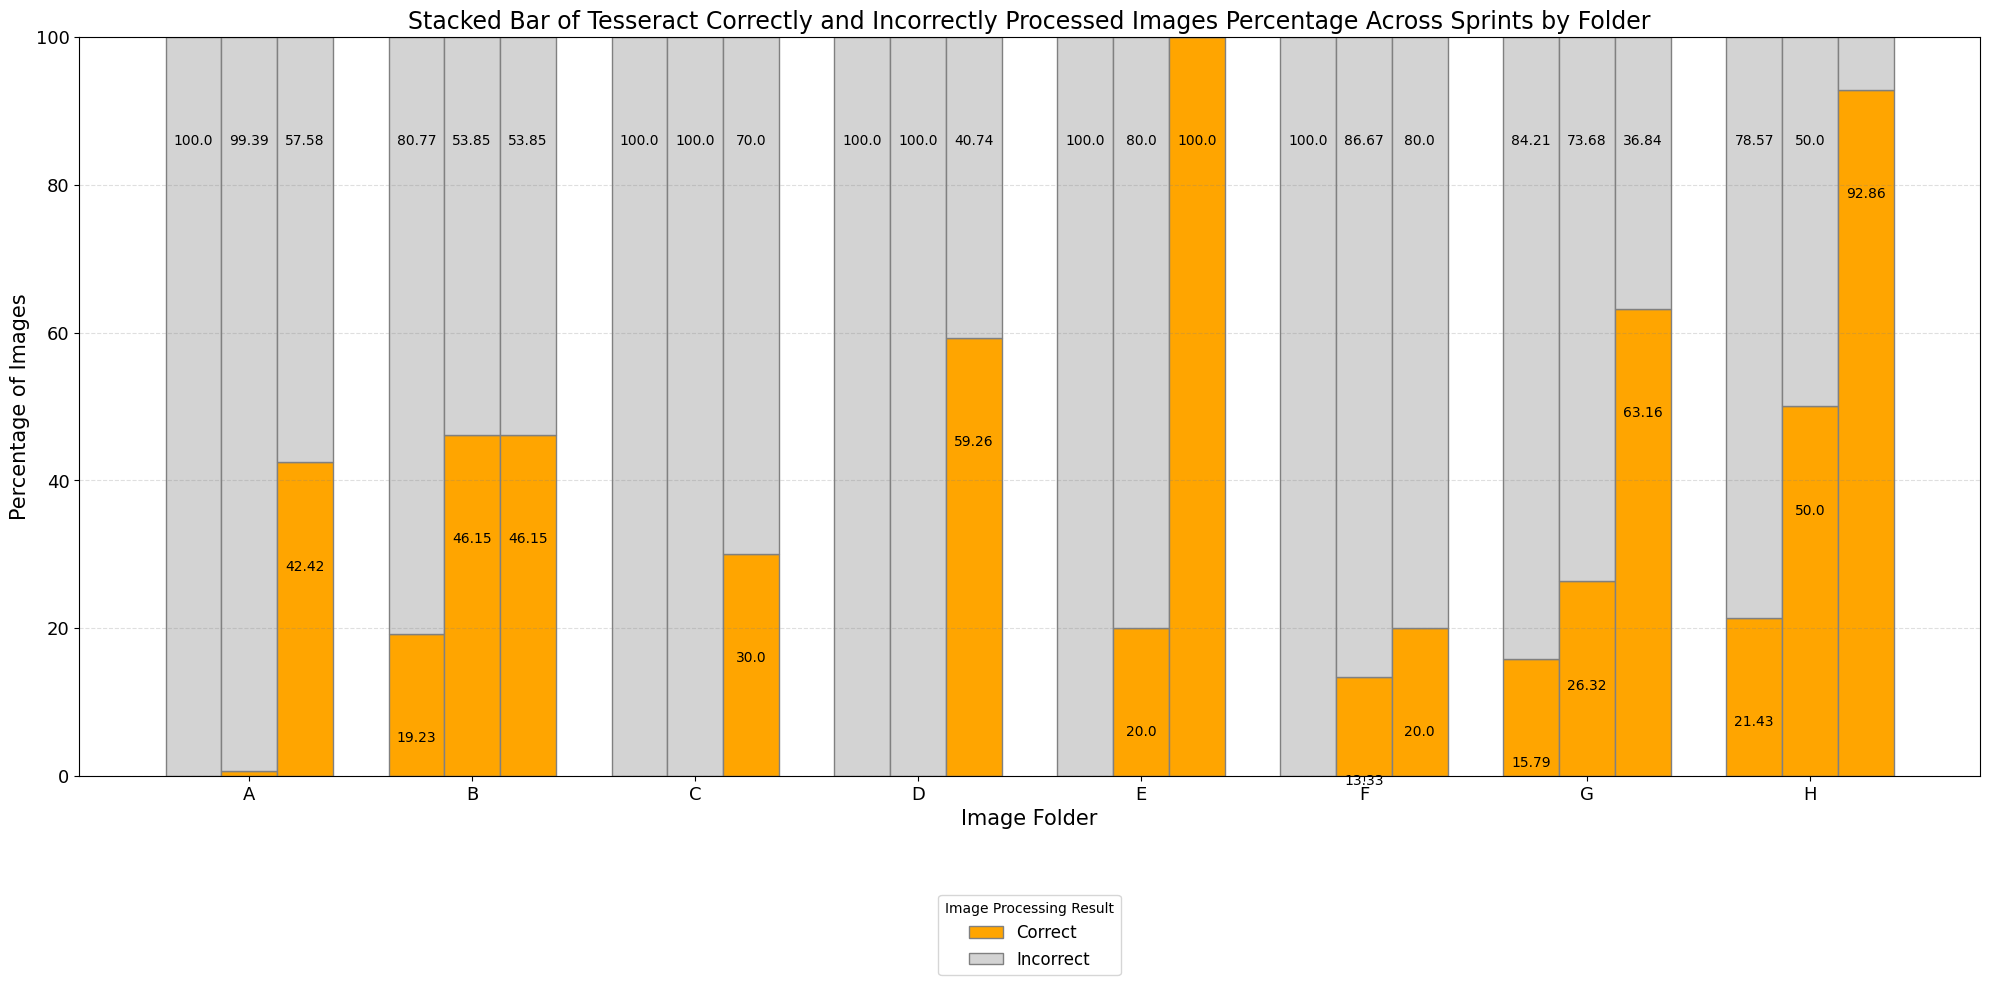
\includegraphics[width=0.9\textwidth]{Figures/Results/tesseract_sprints.png}
    \caption[Tesseract Sprint Results Across Sprints]{Tesseract Sprint Results Across Sprints}
    \label{fig:Tesseract Sprint Results Across Sprints}
\end{figure}

\subsection{Analysis of Image Processing Accuracy Across Sprints}

\subsubsection*{1. Overall Trend}
There is a noticeable improvement in the accuracy of image processing from the ``First Sprint'' to the ``Third Sprint''. This is evident from the increasing size of the darker segments of the bars (representing correctly processed images) across most image folders from one sprint to the next.

\subsubsection*{2. Sprint-wise Observations}
\begin{itemize}
    \item \textbf{First Sprint}: Image processing accuracy is relatively lower, especially for folders A, B, D, and H. Folder G shows a significant number of incorrectly processed images, making it the folder with the highest inaccuracy in this sprint.
    \item \textbf{Second Sprint}: Accuracy has improved across almost all folders, especially for folders A, B, and D. The issues faced during the first sprint for these folders have been addressed. Folder G, however, still has a low accuracy percentage and scope for improvement.
    \item \textbf{Third Sprint}: The accuracy has further improved across all folders. Especially for Folder G, which had a significant number of inaccuracies in the first two sprints, the accuracy has noticeably increased. Folders E, F, and C seem to have almost perfect accuracy in this sprint.
\end{itemize}

\subsubsection*{3. Folder-wise Observations}
\begin{itemize}
    \item \textbf{Folder G}: This folder posed the most significant challenge throughout the sprints. However, by the third sprint, the accuracy improved substantially, indicating that the issues were identified and rectified over time.
    \item \textbf{Folders E, F, and C}: These folders consistently showed high accuracy across all sprints, suggesting that the image processing system was well-tuned for images from these folders from the start.
    \item \textbf{Folder H}: The accuracy for image processing in Folder H has consistently improved across the sprints. Starting with a relatively lower accuracy in the ``First Sprint'', there's a noticeable improvement in the ``Second Sprint'', and by the ``Third Sprint'', the accuracy is near-perfect.
\end{itemize}



\newpage

\section{Fourth Sprint - Analysis CRNN Separate Folders}

\begin{table}[h]
    \centering
    \caption{OCR Performance for CRNN Separate Folders}
    \label{tab:fourth_sprint_results}
    \begin{tabular}{|l|c|c|c|c|}
        \hline
        \textbf{Folder} & \textbf{Total Count} & \multicolumn{3}{c|}{\textbf{CRNN}}                                            \\
        \hline
                        &                      & \textbf{Read}                      & \textbf{Not Read} & \textbf{No Contours} \\
        \hline
        A               & 165                  & 46                                 & 9                 & 105                  \\
        B               & 26                   & 17                                 & 9                 & 0                    \\
        C               & 10                   & 1                                  & 8                 & 1                    \\
        D               & 27                   & 1                                  & 4                 & 6                    \\
        E               & 10                   & 4                                  & 6                 & 0                    \\
        F               & 15                   & 0                                  & 6                 & 8                    \\
        G               & 19                   & 17                                 & 2                 & 0                    \\
        H               & 14                   & 6                                  & 7                 & 1                    \\
        \hline
    \end{tabular}
\end{table}
\vspace{1in}
Of the 286 images 92 were read making a 32.16\% read count.
\vspace{1in}
\begin{figure}[ht]
    \centering
    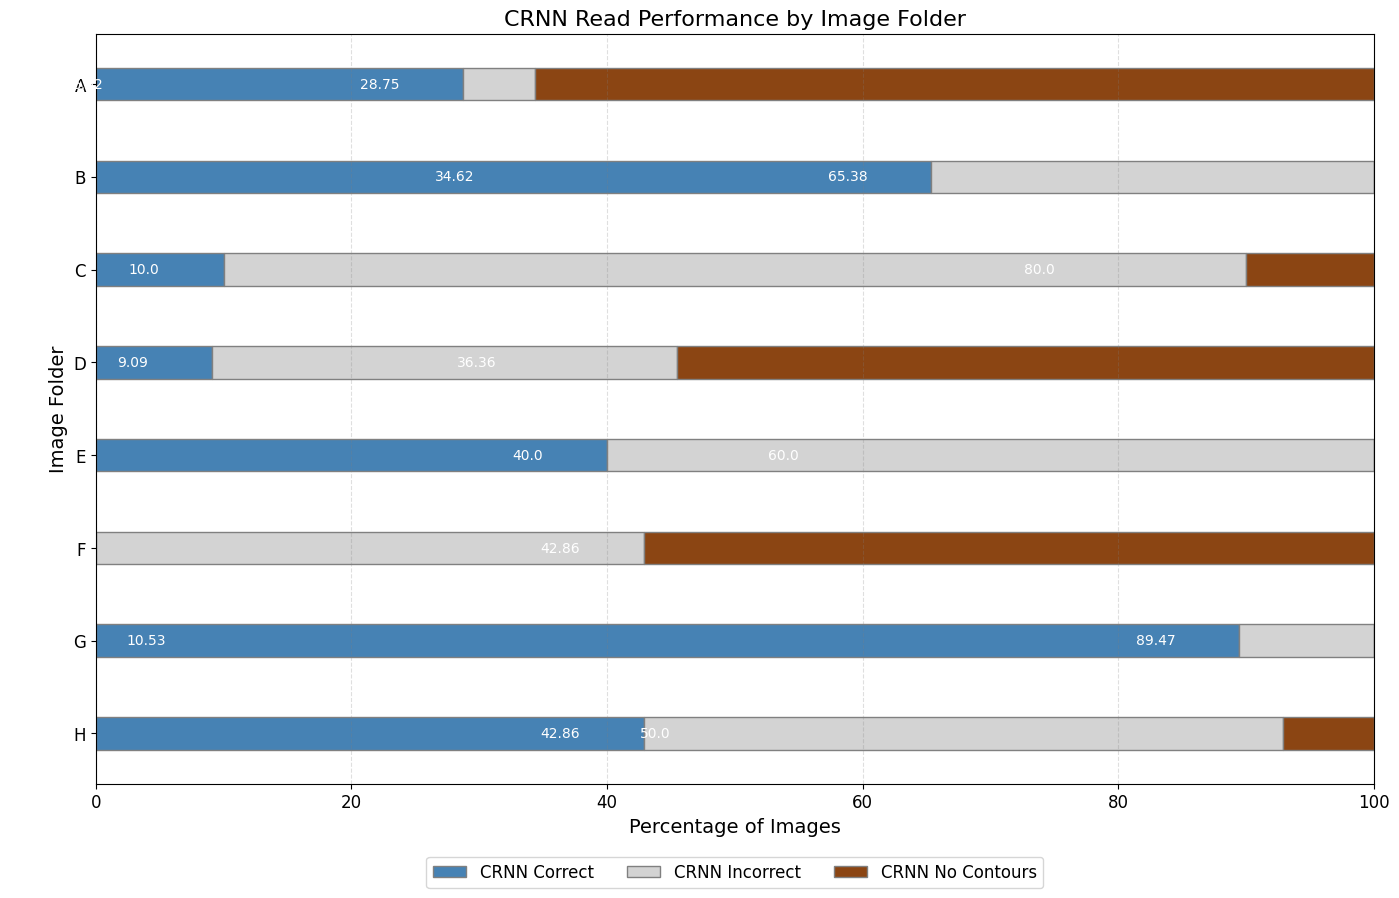
\includegraphics[width=0.99\textwidth]{Figures/Results/crnn.png}
    \caption[CRNN Results]{CRNN Results}
    \label{fig:CRNN Results}
\end{figure}

\newpage

\section{Tesseract and CRNN Combined}

\begin{table}[h]
    \centering
    \caption{OCR Performance for Different Folders}
    \label{tab:ocr_performance}
    \begin{tabular}{|l|c|c|c|c|c|c|}
        \hline
        \textbf{Folder} & \textbf{Total Count} & \multicolumn{2}{c|}{\textbf{Tesseract}} & \multicolumn{3}{c|}{\textbf{CRNN}}                                                            \\
        \hline
                        &                      & \textbf{Read}                           & \textbf{Not Read}                  & \textbf{Read} & \textbf{Not Read} & \textbf{No Contours} \\
        \hline
        A               & 165                  & 70                                      & 90                                 & 46            & 9                 & 105                  \\
        B               & 26                   & 12                                      & 14                                 & 17            & 9                 & 0                    \\
        C               & 10                   & 3                                       & 7                                  & 1             & 8                 & 1                    \\
        D               & 27                   & 16                                      & 11                                 & 1             & 4                 & 6                    \\
        E               & 10                   & 10                                      & 0                                  & 4             & 6                 & 0                    \\
        F               & 15                   & 1                                       & 14                                 & 0             & 6                 & 8                    \\
        G               & 19                   & 12                                      & 7                                  & 17            & 2                 & 0                    \\
        H               & 14                   & 13                                      & 1                                  & 6             & 7                 & 1                    \\
        \hline
    \end{tabular}
\end{table}
\vspace{1.5in}
\begin{figure}[ht]
    \centering
    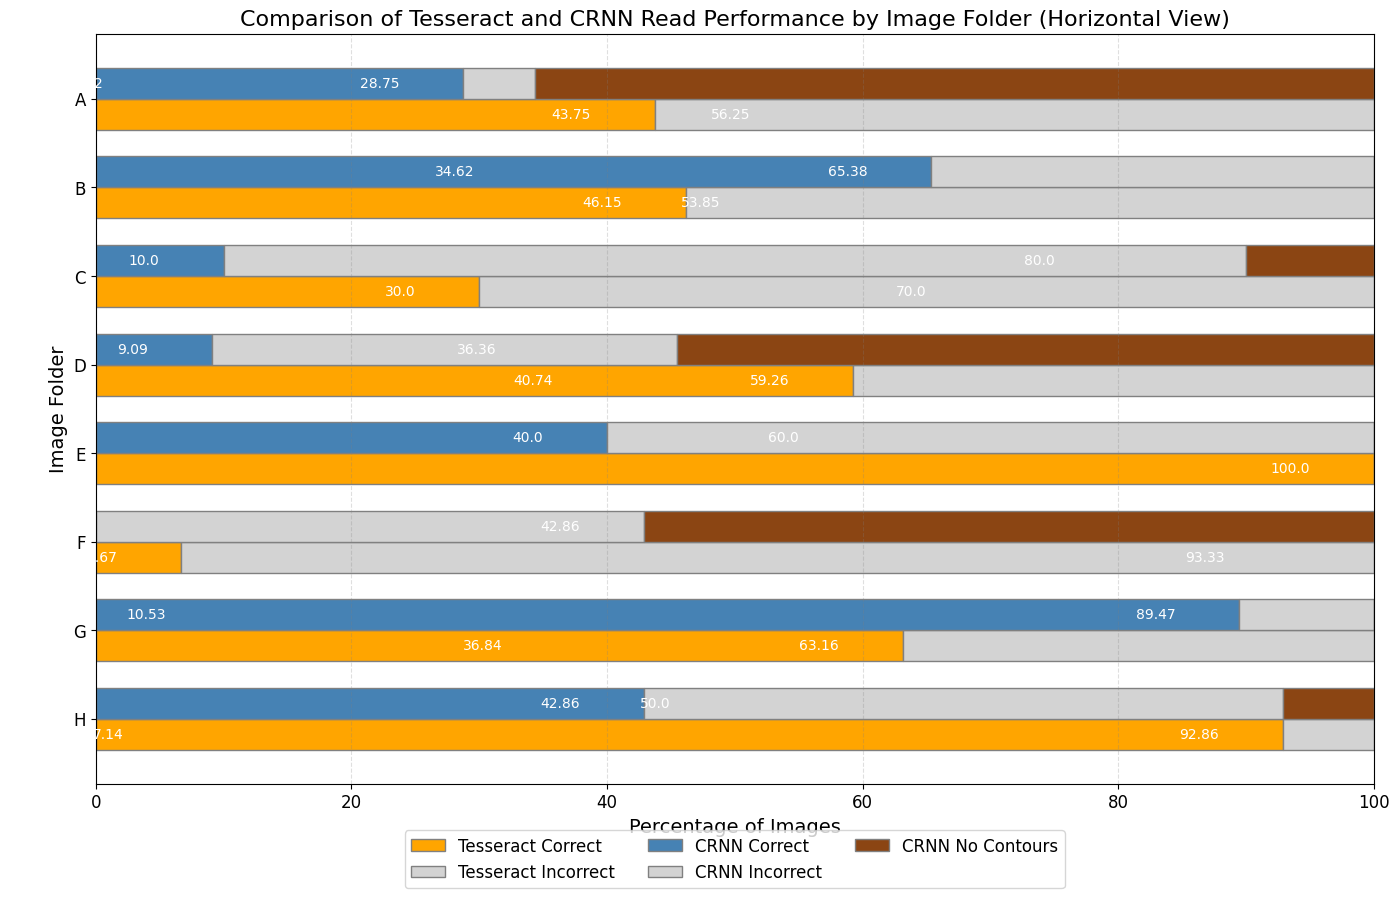
\includegraphics[width=0.99\textwidth]{Figures/Results/tesseract_vs_crnn.png}
    \caption[Tesseract Versus CRNN]{Tesseract Versus CRNN}
    \label{fig:Tesseract Versus CRNN}
\end{figure}

\newpage


\subsection{Analysis of Tesseract and CRNN Performance}

\begin{enumerate}
    \item \textbf{Overall Performance}:
          \begin{itemize}
              \item \textbf{Tesseract}: Tesseract showcases consistent performance across most image folders. Notably, folders E and H both achieve an accuracy above 90\%.
              \item \textbf{CRNN}: CRNN's performance varies extensively across the folders. In Folder A, its read percentage is only 28.75\%, indicating a significant area for improvement.
          \end{itemize}

    \item \textbf{Image Folder Specific Insights}:
          \begin{itemize}
              \item \textbf{Folder A}: Tesseract significantly outperforms CRNN.
              \item \textbf{Folder B}: CRNN outperforms Tesseract.
              \item \textbf{Folder C}: Tesseract has a distinct advantage over CRNN albeit the performance both is poor.
              \item \textbf{Folder D}: Tesseract performs better, while CRNN struggles, especially with contour detection.
              \item \textbf{Folder E}: Tesseract achieves an impressive accuracy rate of 100\%, surpassing CRNN.
              \item \textbf{Folder F}: Tesseract and CRNN perform poorly, notably in contour detection.
              \item \textbf{Folder G}: CRNN outperforms Tesseract.
              \item \textbf{Folder H}: Tesseract achieves another outstanding accuracy rate of over 90\%, significantly outperforming CRNN.
          \end{itemize}

    \item \textbf{CRNN's Contour Detection}:
          \begin{itemize}
              \item A significant challenge for CRNN is its inability to detect contours, especially evident in folders A and D. This indicates a potential area for improvement or adjustment in the CRNN model for specific image types.
          \end{itemize}

    \item \textbf{Comparison}:
          \begin{itemize}
              \item Tesseract has outperformed CRNN in all folders apart from B and G. On the other hand, while CRNN exhibits potential in some folders, its variable performance and specific challenges in others highlight areas that need addressing.
          \end{itemize}

\end{enumerate}

In conclusion, Tesseract's performance is higher, especially in folders E and H, makes it a preferable choice in its current state. CRNN, with its present inconsistencies, requires further tuning or modifications for enhanced reliability.



